\documentclass[11pt]{article}

\usepackage[margin=1in]{geometry}
\usepackage{amsmath,amssymb}
\usepackage{newtxtext,newtxmath}
\usepackage{booktabs}
\usepackage{graphicx}
\usepackage{float}
\usepackage{placeins}
\usepackage{url}
\usepackage[hidelinks]{hyperref}

\begin{document}

\thispagestyle{empty}
\vspace*{0.5cm}

\noindent\rule{\textwidth}{2pt}

\vspace{0.45cm}
\begin{center}
  {\LARGE\bfseries Superposition Geometry as a Training Signal}
\end{center}
\vspace{0.35cm}

\noindent\rule{\textwidth}{0.8pt}

\vspace{0.6cm}

\begin{center}
\begin{minipage}[t]{0.3\textwidth}
\centering
{\bfseries Ash Manvi}\par
Aquin Labs\par
{\ttfamily ash@aquin.app}
\end{minipage}
\hfill
\begin{minipage}[t]{0.3\textwidth}
\centering
{\bfseries Samreena Tajreen}\par
Aquin Labs\par
{\ttfamily samreena@aquin.app}
\end{minipage}
\end{center}

\vspace{0.55cm}

\begin{center}
  {\Large\bfseries Abstract}
\end{center}

\begin{quote}
Loss tells you how wrong a model is. It does not tell you how tangled the
features became while it got less wrong. Language models store more features
than they have dimensions; that sharing is superposition, and its shape
(who interferes with whom, how energy spreads across local modes) is
superposition geometry. We treat that geometry the way trainers already treat
loss: as a live signal printed every step, and as something you can gently
push.

On Qwen2.5-7B fine-tunes we log interference, spectral participation, and
coactivation beside the loss curve across layers. The curves move with
training: mid layers keep related facts close and unrelated facts far; late
layers show a sharp spectral phase change that loss alone never shows. We then
add a soft regularizer on one mid-layer interference toward a packing target
$m^\star{=}0.35$. In a matched seed-0 pair the controlled run lands closer to
the target, improves held-out LM loss, preserves cross-feature structure, and
passes a seven-claim out-of-metric validation suite. Scaling from 1.5B to 7B
turns a packing-only win into a packing \emph{and} held-out win.

The claim is practical. Geometry belongs on the training dashboard. Soft
control is a real knob, not a slogan. Code, configs, and figures ship with the
paper at
\url{https://github.com/Aquinf03/superposition-geometry-signal}.
\end{quote}

\section{Introduction}

Watch a training run and you almost always watch one number: loss. Loss is
honest about prediction error. It is quiet about representation shape. Two
runs can finish with similar loss and very different packing: how tightly
features sit on top of each other, which layers collapsed into a few modes,
which neighborhoods stayed clean.

That packing is not a side curiosity. Toy models already showed that neural
nets store more features than dimensions by sharing directions in
superposition~\cite{elhage2022toy}. Follow-on work maps monosemantic features
with dictionaries~\cite{bricken2023monosemanticity}, studies spectral
geometry of interference~\cite{ivanov2026spectral}, and asks which connections
are compromise rather than pure signal~\cite{olah2025interference}. Most of
that work is post-hoc: freeze a model, dig, report. Training itself still
looks like a loss curve.

We put geometry on the same cadence as loss:
\begin{quote}
\emph{Can we track how features pack while a model trains, layer by layer,
step by step, and then softly steer that packing without wrecking the run?}
\end{quote}
Yes. Section~\ref{sec:method} defines three cheap local metrics and a soft
control term. Section~\ref{sec:watch} shows what the live dashboard reveals on
a real 7B fine-tune. Section~\ref{sec:control} turns the knob and checks the
run with out-of-metric tests. Section~\ref{sec:limits} says where the signal
lies and how to read it.

\section{What we do}
\label{sec:method}

The recipe is short on purpose (Figure~\ref{fig:live}).

\begin{figure}[H]
  \centering
  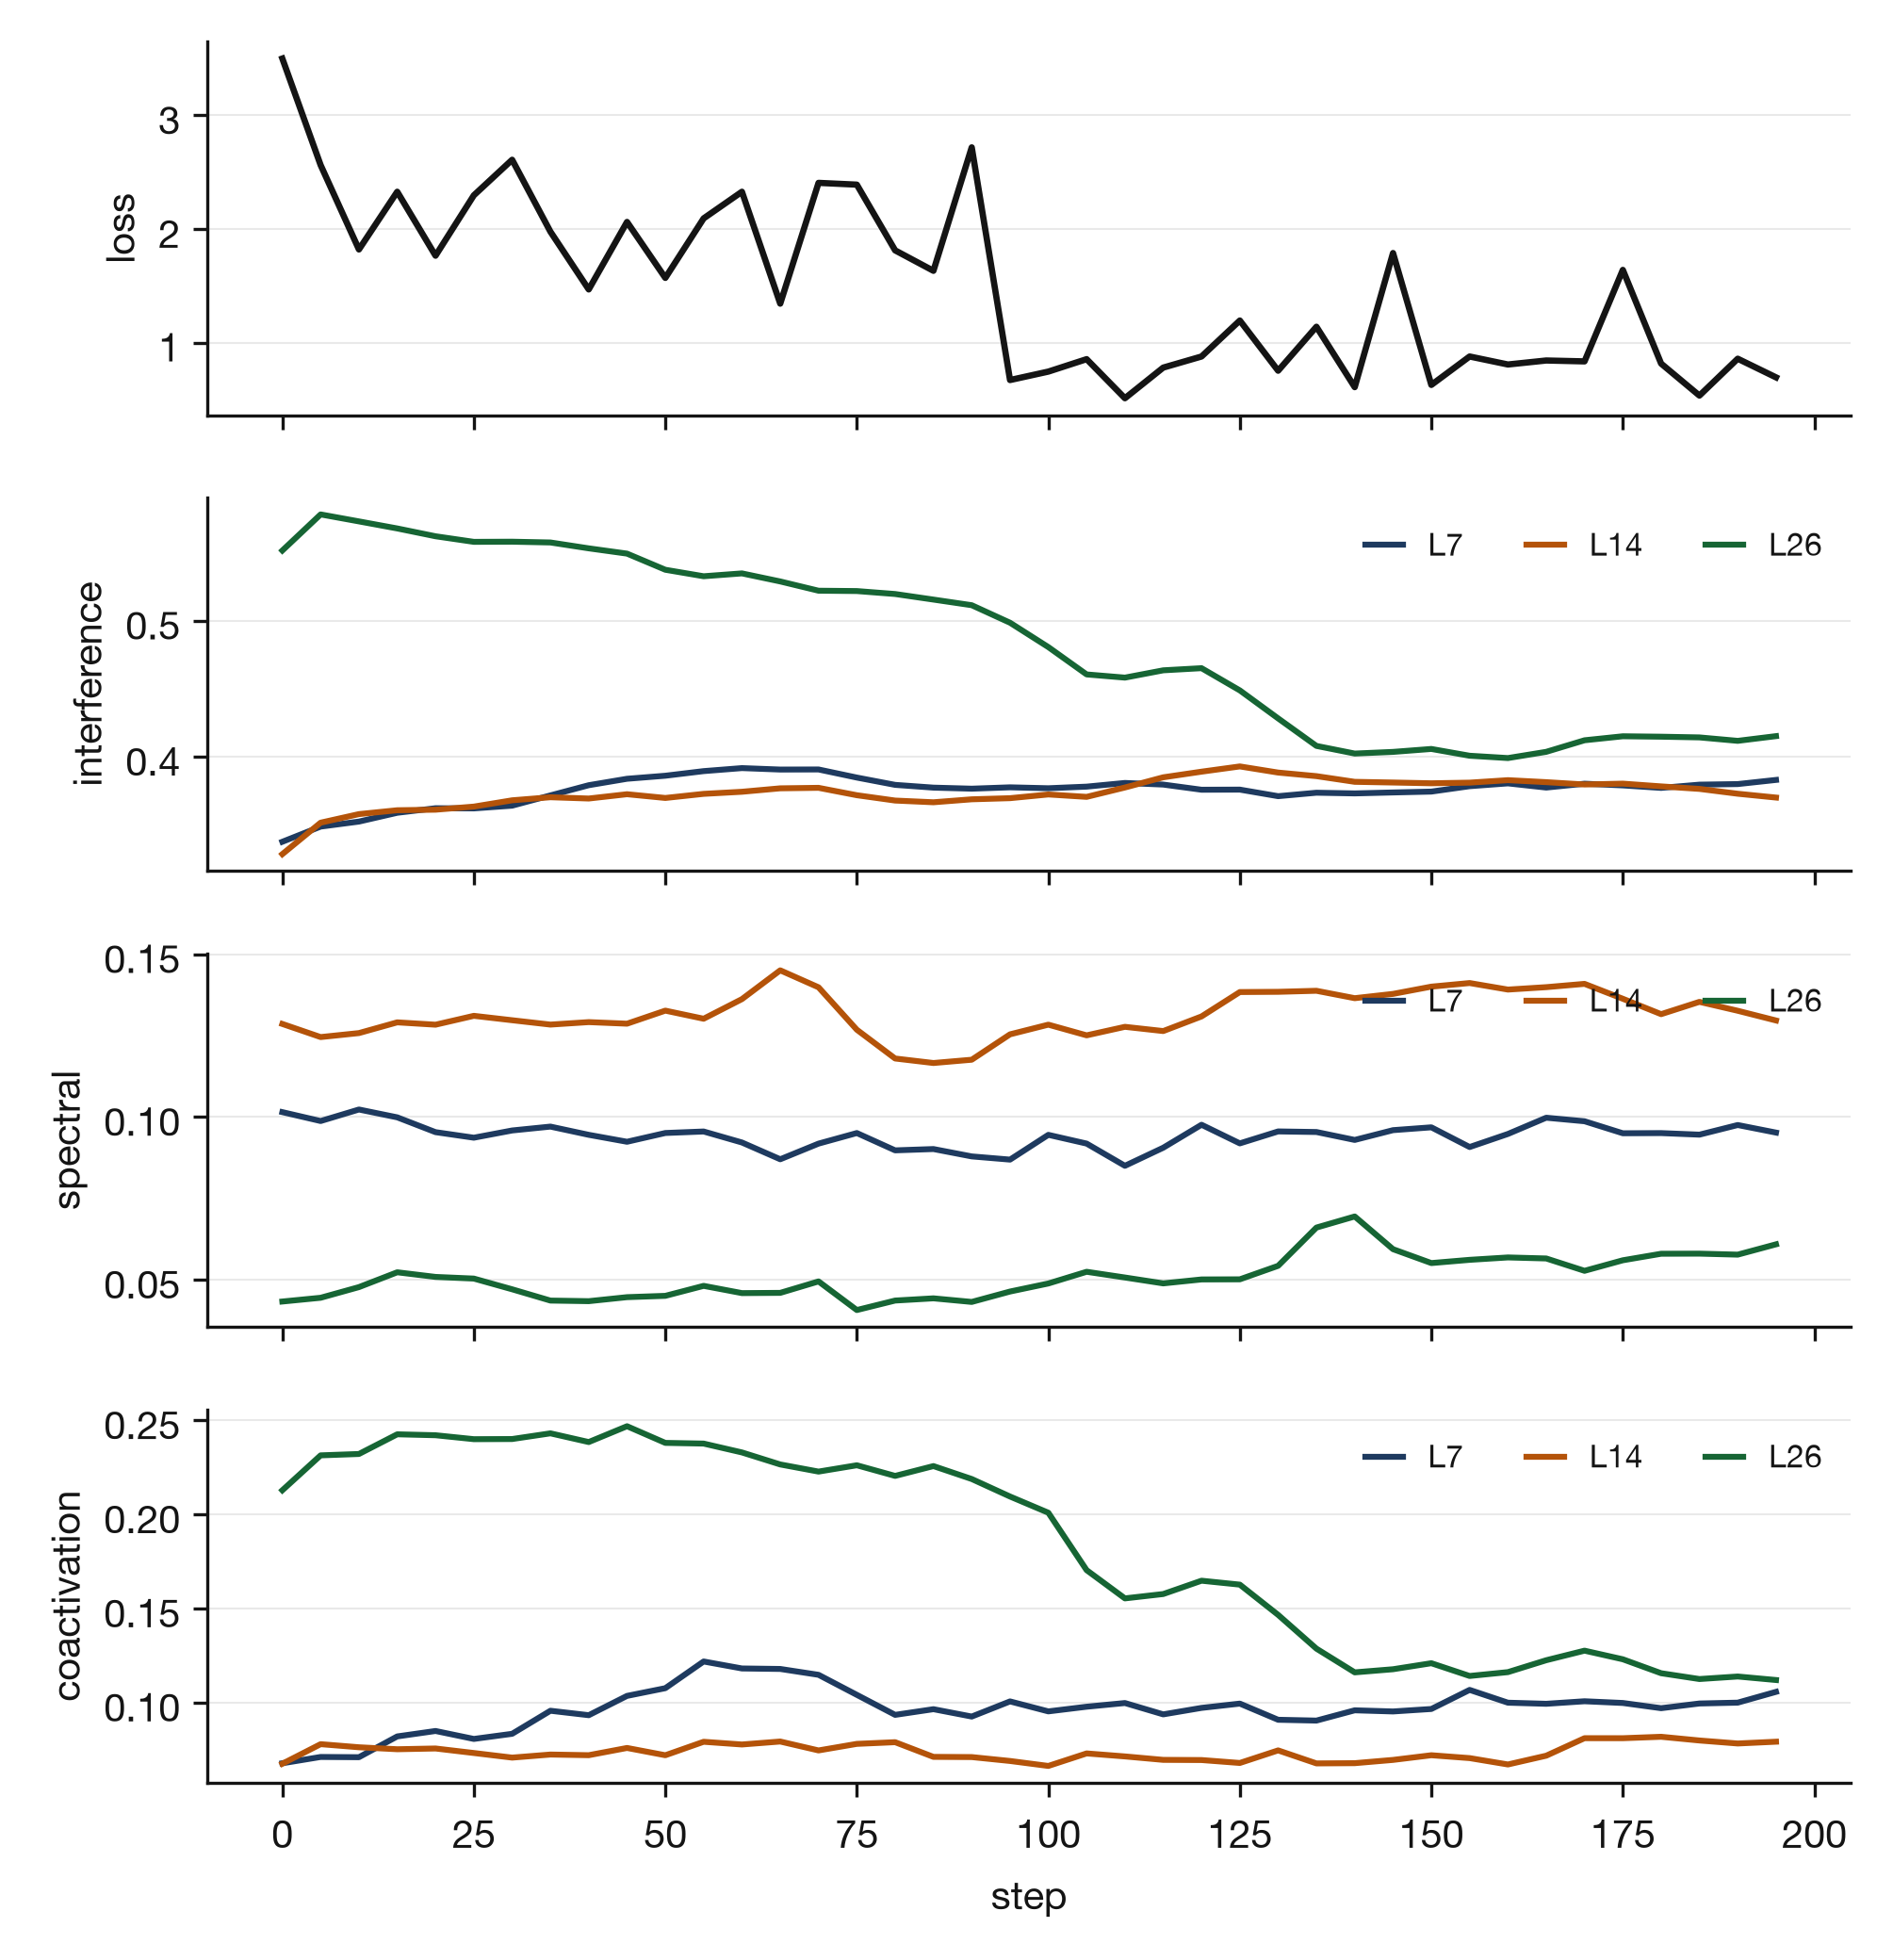
\includegraphics[width=\linewidth]{figures/fig01_live_track.png}
  \caption{The idea on the dashboard: run once, print loss beside multi-layer
  geometry every few steps, then (optionally) softly steer packing toward a
  target.}
  \label{fig:live}
\end{figure}

\paragraph{Probe a bank, score a query.}
At chosen MLP-out layers we build a neighbor bank from a fixed probe prompt
set (TransformerLens hooks~\cite{nanda2022transformerlens}). For a query
activation we score three local geometry quantities:

\begin{itemize}
  \item \textbf{Interference:} mean absolute cosine to the top-$k$
  neighbors. High means the query sits near many other directions.
  \item \textbf{Spectral participation:} how the query's energy spreads
  across eigenvectors of the neighbor covariance, normalized to $[0,1]$.
  Near $0$ is localized; near $1$ is more superposition-like.
  \item \textbf{Coactivation:} average Jaccard overlap of top-activated
  coordinates between query and each neighbor (capped to roughly $d/4$ dims
  so dense vectors cannot trivially score $1$).
\end{itemize}

\paragraph{Print it beside loss.}
Every logging step the trainer emits a single line:
\begin{center}
\texttt{step=12  loss=0.41  |  geometry: interference=\ldots\ spectral=\ldots\ coact=\ldots}
\end{center}
Multi-layer runs write \texttt{geometry\_L\{n\}\_*} columns into a CSV and
freeze a geometry sidecar next to every weight checkpoint, so later diffs use
the same probes and layers.

\paragraph{Diff features, not just scalars.}
Scalars say the tangle moved. Feature diffs say \emph{what} moved. We compare
neighborhoods across checkpoints and across feature pairs at the same step:
related location prompts (Eiffel vs Louvre) versus an unrelated pair. Mid
layers should keep related close and unrelated far; that is structure you can
see.

\paragraph{Soft control.}
Geometry also gets a knob. Pick one layer, one metric, one target, and add
\[
\mathcal{L} \;=\; \mathcal{L}_{\mathrm{LM}}
  \;+\; \lambda\,(\,m - m^\star\,)^2
\]
after a short warmup where $\lambda{=}0$ and the live signal must already be
moving. Band and feature-relative variants exist in the SDK; this paper's
matched pair uses the point target. Control is off by default.

That is the whole loop: watch, diff, optionally steer, validate.
\FloatBarrier

\section{What the watch shows}
\label{sec:watch}

We fine-tune Qwen2.5-7B for $200$ steps on an extended factual corpus
(seed $0$, bf16), tracking layers $7$, $14$, and $26$. Loss falls from about
$3.5$ to $0.43$. Geometry does not sit still while that happens.

\subsection{Layers disagree on purpose}

Figure~\ref{fig:phase} plots spectral participation by layer. Late layer $26$
swings early then settles on a different path from the mid layers, a phase
pattern invisible if you only plot loss. Mid layers drift differently from
each other too. The dashboard's job is exactly this: show that training is
not one curve.

\begin{figure}[H]
  \centering
  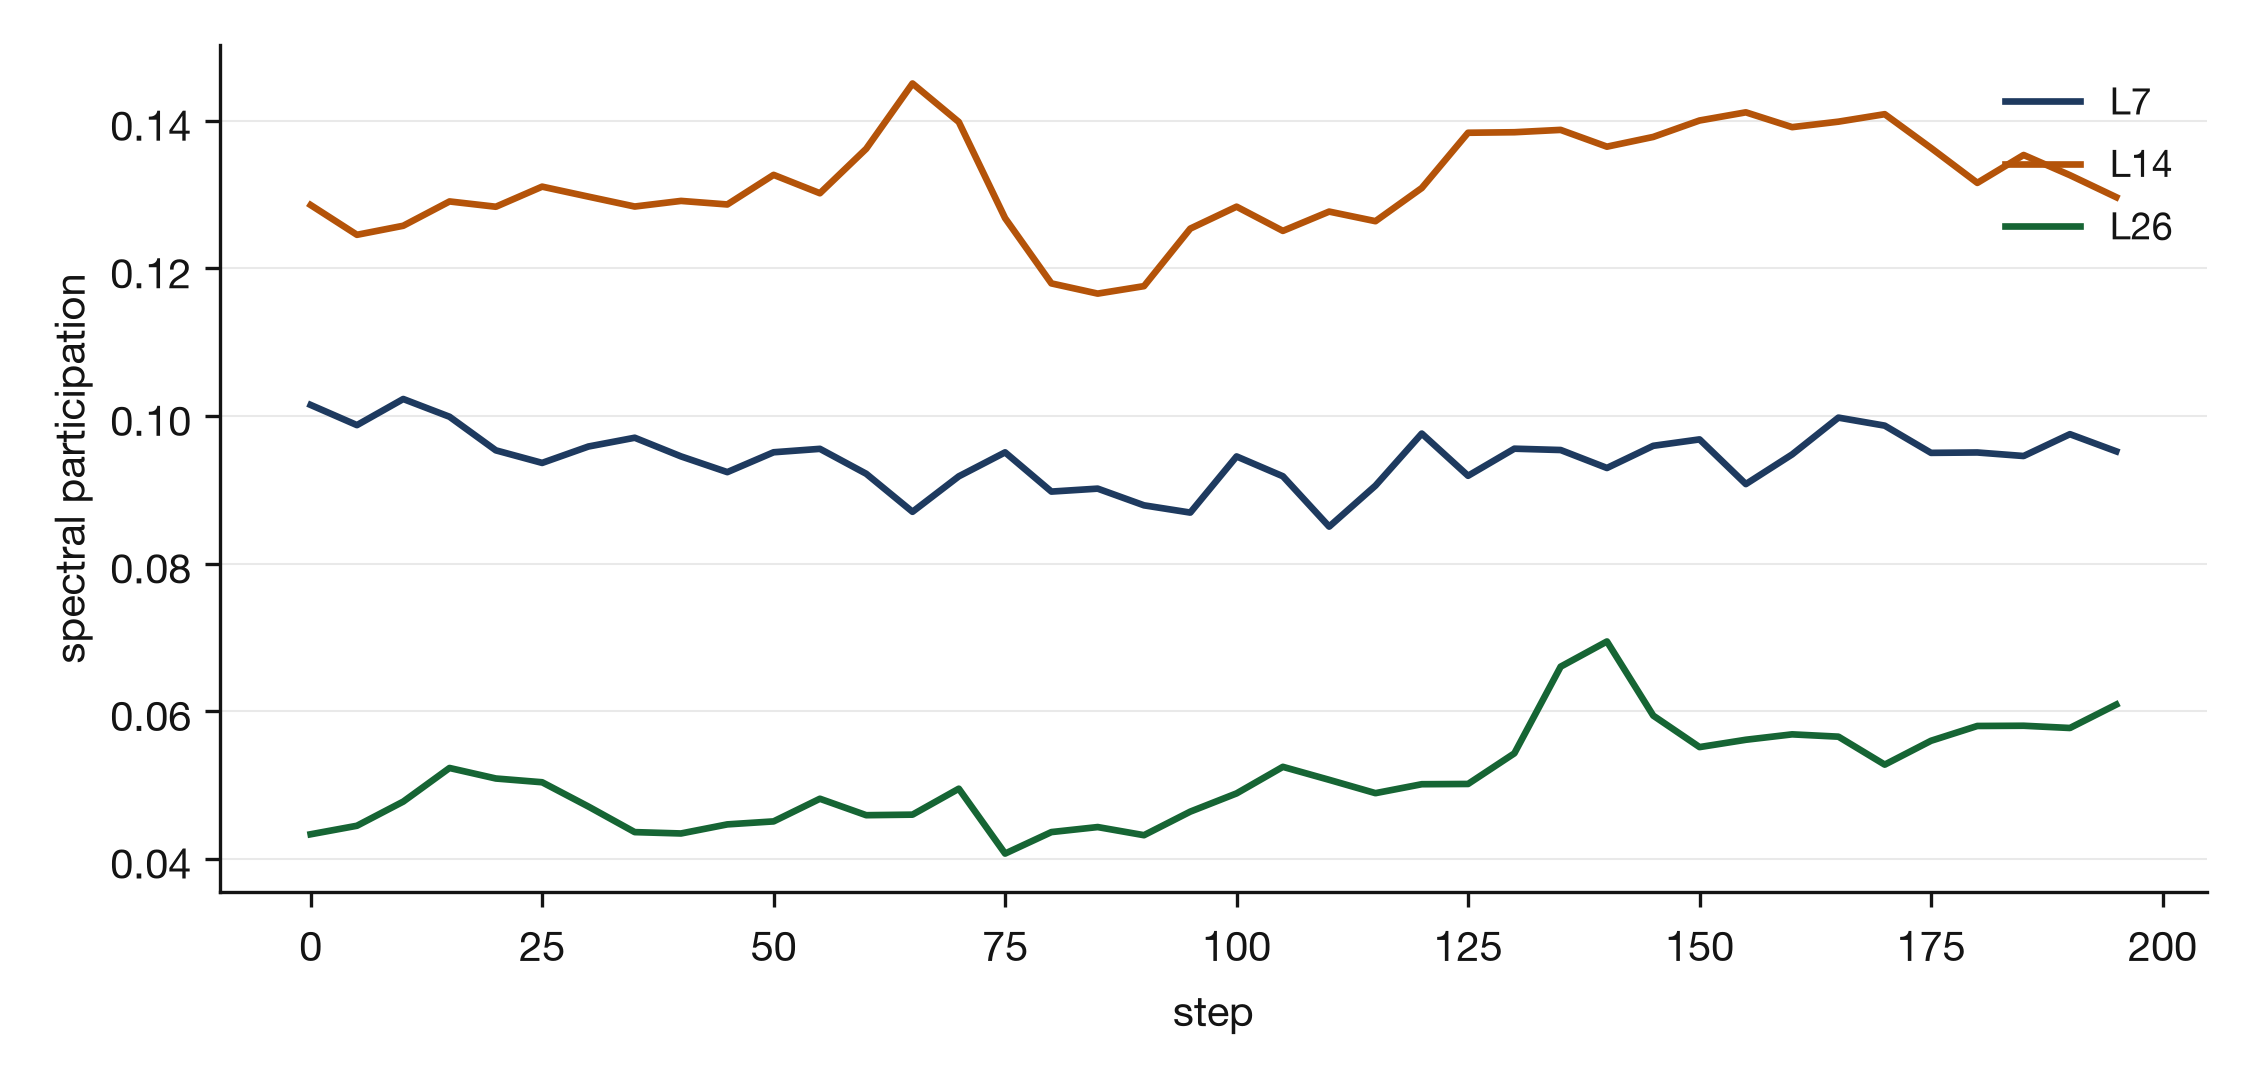
\includegraphics[width=0.92\linewidth]{figures/fig03_layer_phase.png}
  \caption{Spectral participation by layer over the $200$-step Qwen2.5-7B run.
  Layers disagree on timing and direction; a loss-only plot would miss that.}
  \label{fig:phase}
\end{figure}

\subsection{Related stays closer than unrelated}

At step $199$, cross-feature neighborhood deltas at mid layers separate cleanly
(Figure~\ref{fig:cross}): related location features score about $0.037$ apart;
an unrelated pair sits near $0.280$.

\begin{figure}[H]
  \centering
  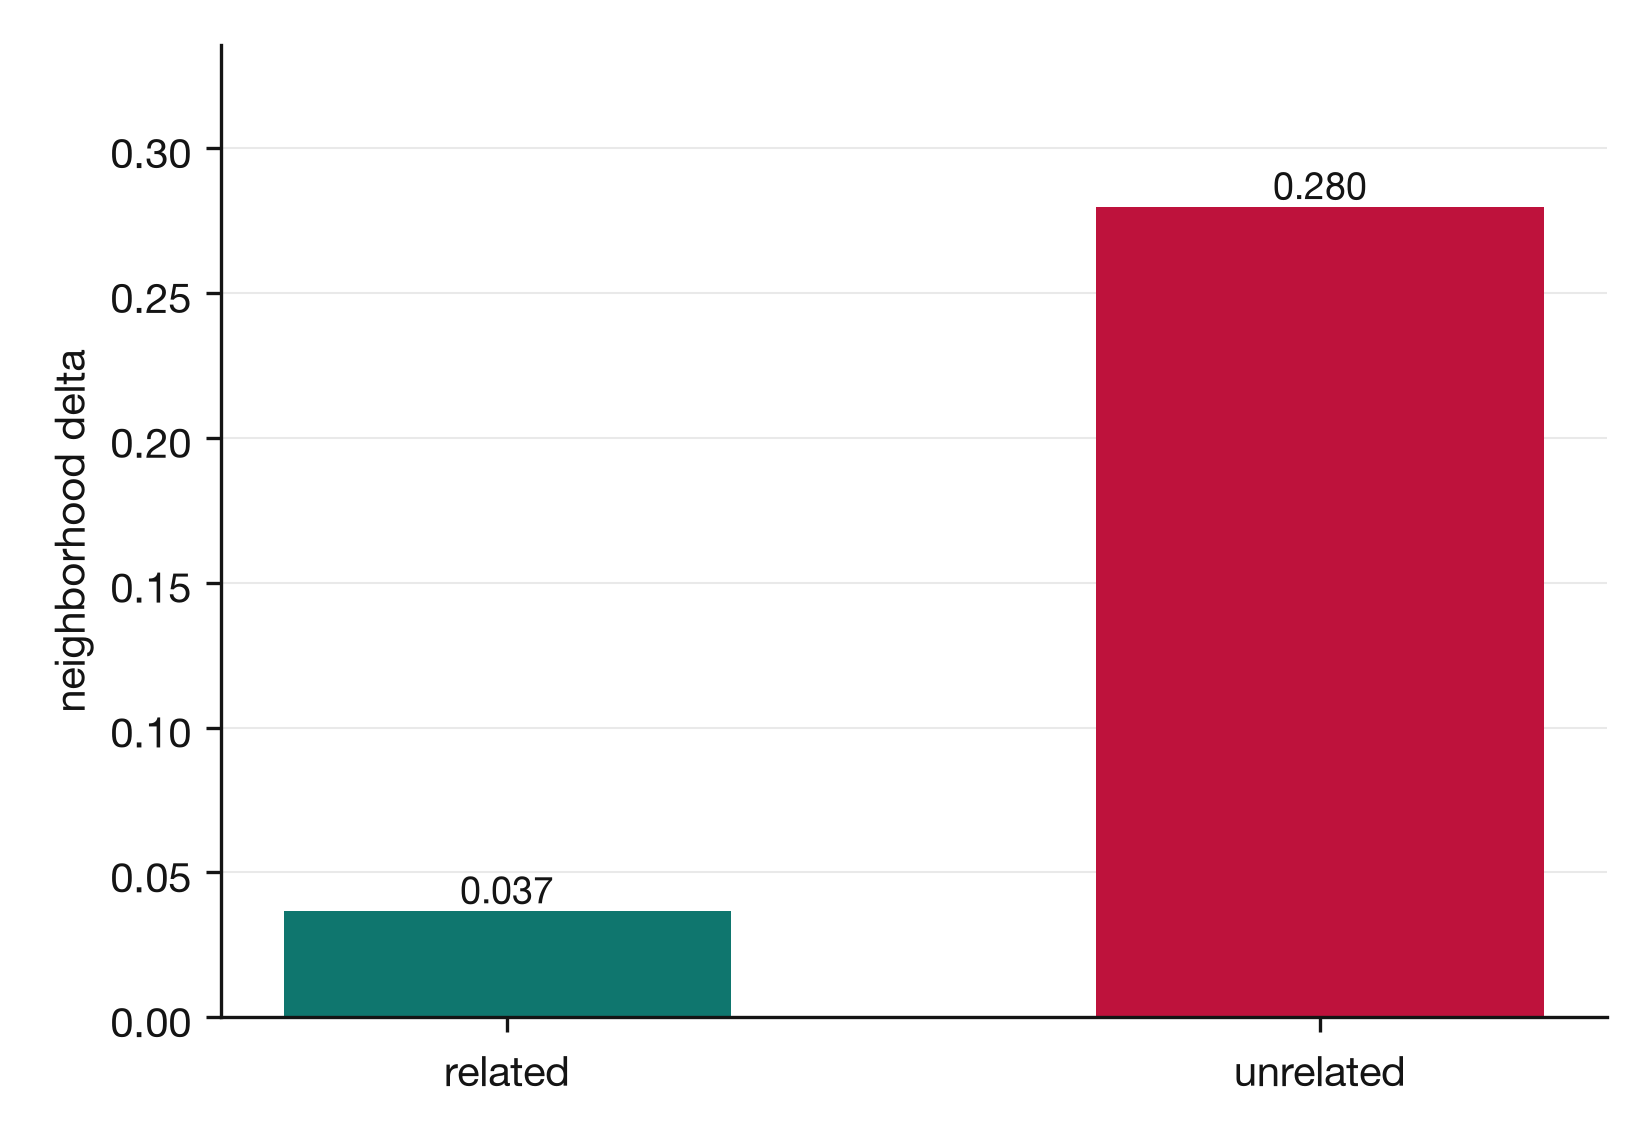
\includegraphics[width=0.92\linewidth]{figures/fig04_cross_feature.png}
  \caption{Cross-feature neighborhood deltas at mid layers (step $199$).
  Related location features stay far closer than unrelated pairs.}
  \label{fig:cross}
\end{figure}

Figure~\ref{fig:stills} shows the same contrast as neighborhood stills. We
read structure at mid layers; late-layer spectra are treated as a phase
marker rather than the place to score relatedness.

\begin{figure}[H]
  \centering
  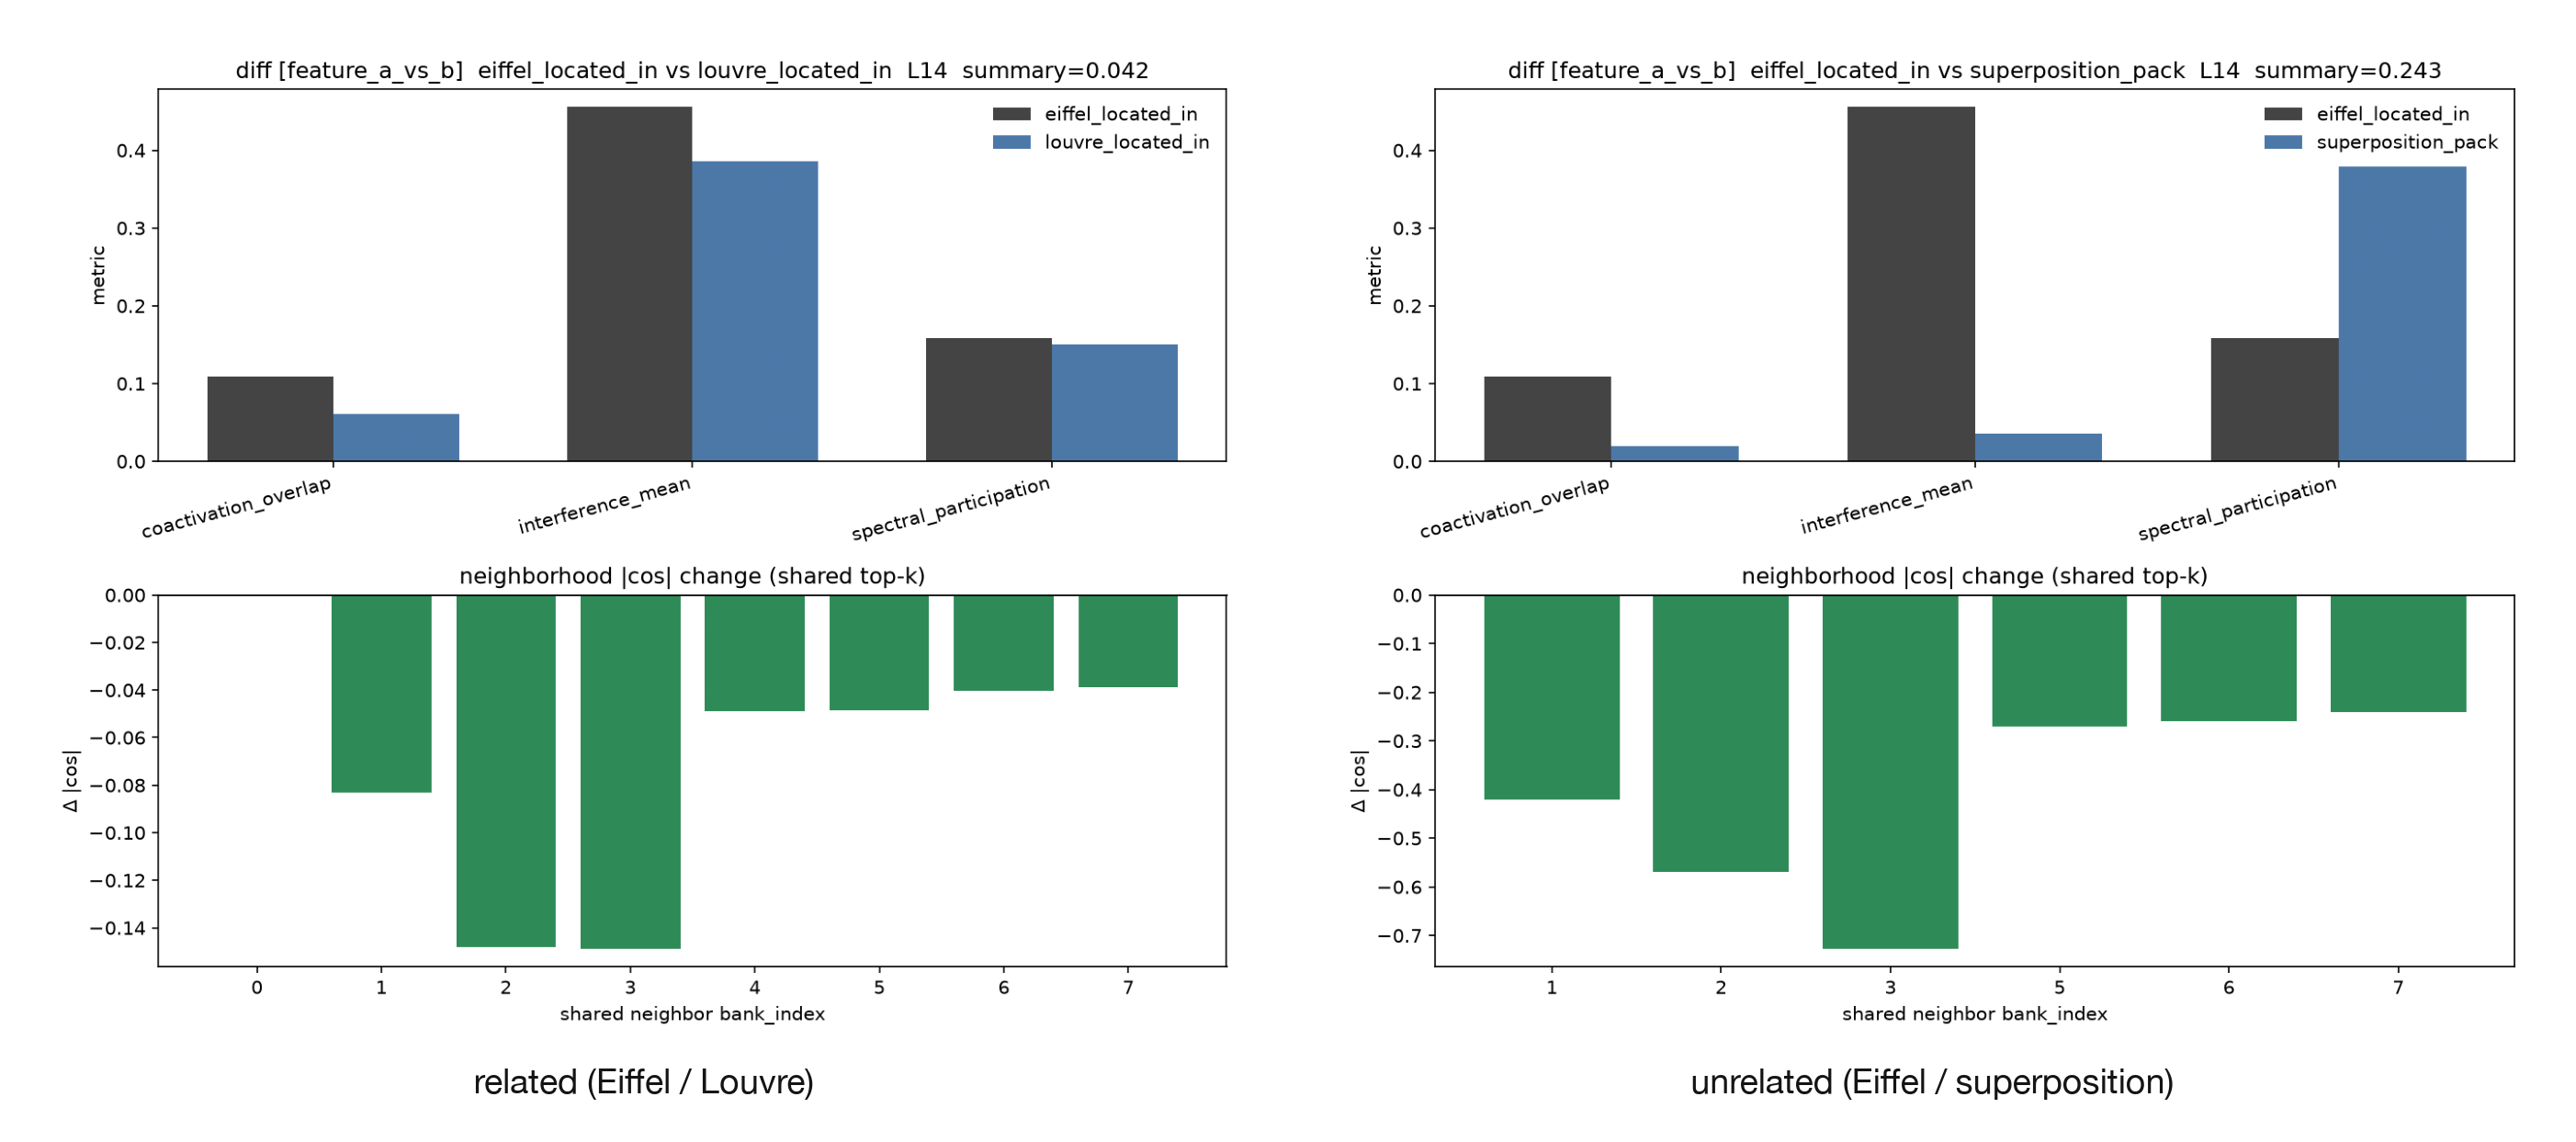
\includegraphics[width=\linewidth]{figures/fig07_neighborhood_stills.png}
  \caption{Neighborhood stills at step $199$, L14: related feature pair (left)
  versus unrelated pair (right).}
  \label{fig:stills}
\end{figure}

Figure~\ref{fig:view} is the live \texttt{spg view} scrubber on the same run:
neighborhoods morph from step $0$ to step $195$ while you scrub layers and time.

\begin{figure}[H]
  \centering
  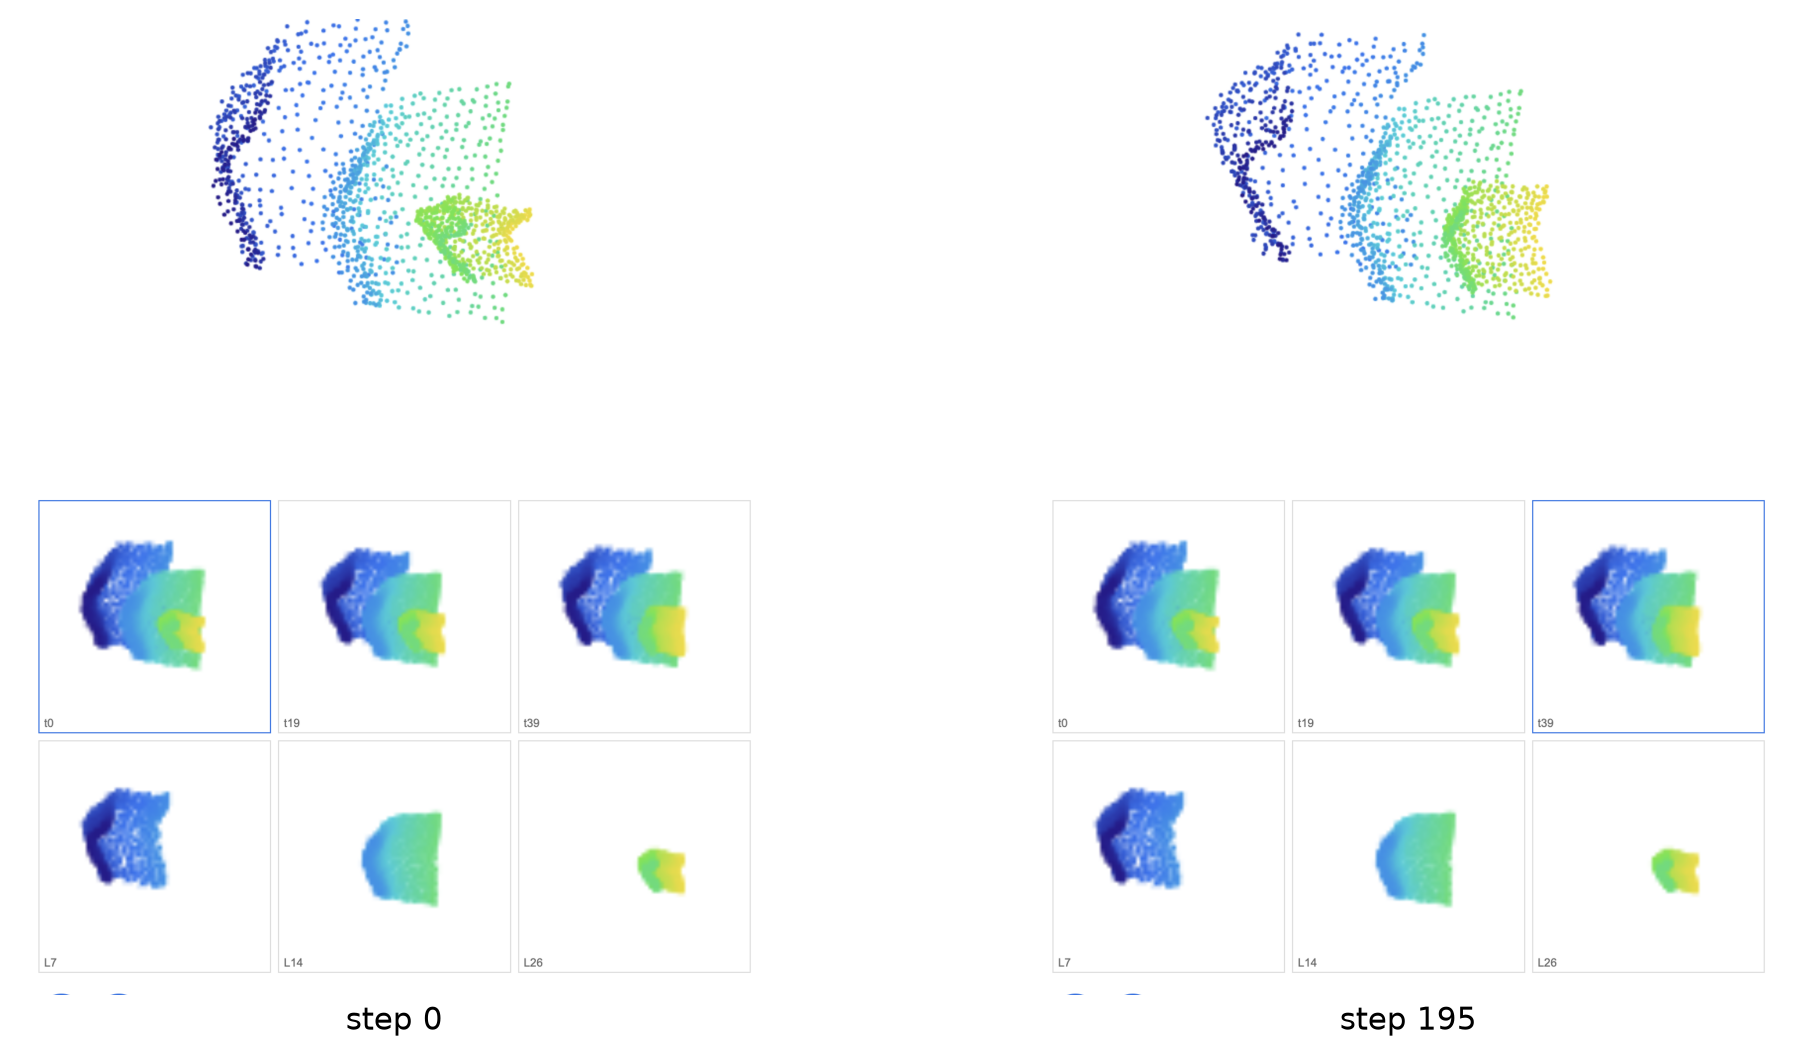
\includegraphics[width=\linewidth]{figures/fig08_view_morph.png}
  \caption{\texttt{spg view} neighborhood morph on the Qwen2.5-7B run (L14).
  Left: step $0$. Right: step $195$. The interactive HTML scrubber ships with
  the SDK.}
  \label{fig:view}
\end{figure}

The watch signal is doing useful work: it moves with training, splits by
layer, and respects feature relatedness. That is enough to put it on the
dashboard.
\FloatBarrier

\section{Turning the knob}
\label{sec:control}

Watching is half the product. The other half is control. We match seed, corpus,
model, steps, and learning rate, then enable a soft regularizer on L14
interference toward $m^\star{=}0.35$ with $\lambda{=}5{\times}10^{-2}$ and $20$
warmup steps (Figure~\ref{fig:control}). Watch and control share the full probe
bank and the same logging cadence.

\begin{figure}[H]
  \centering
  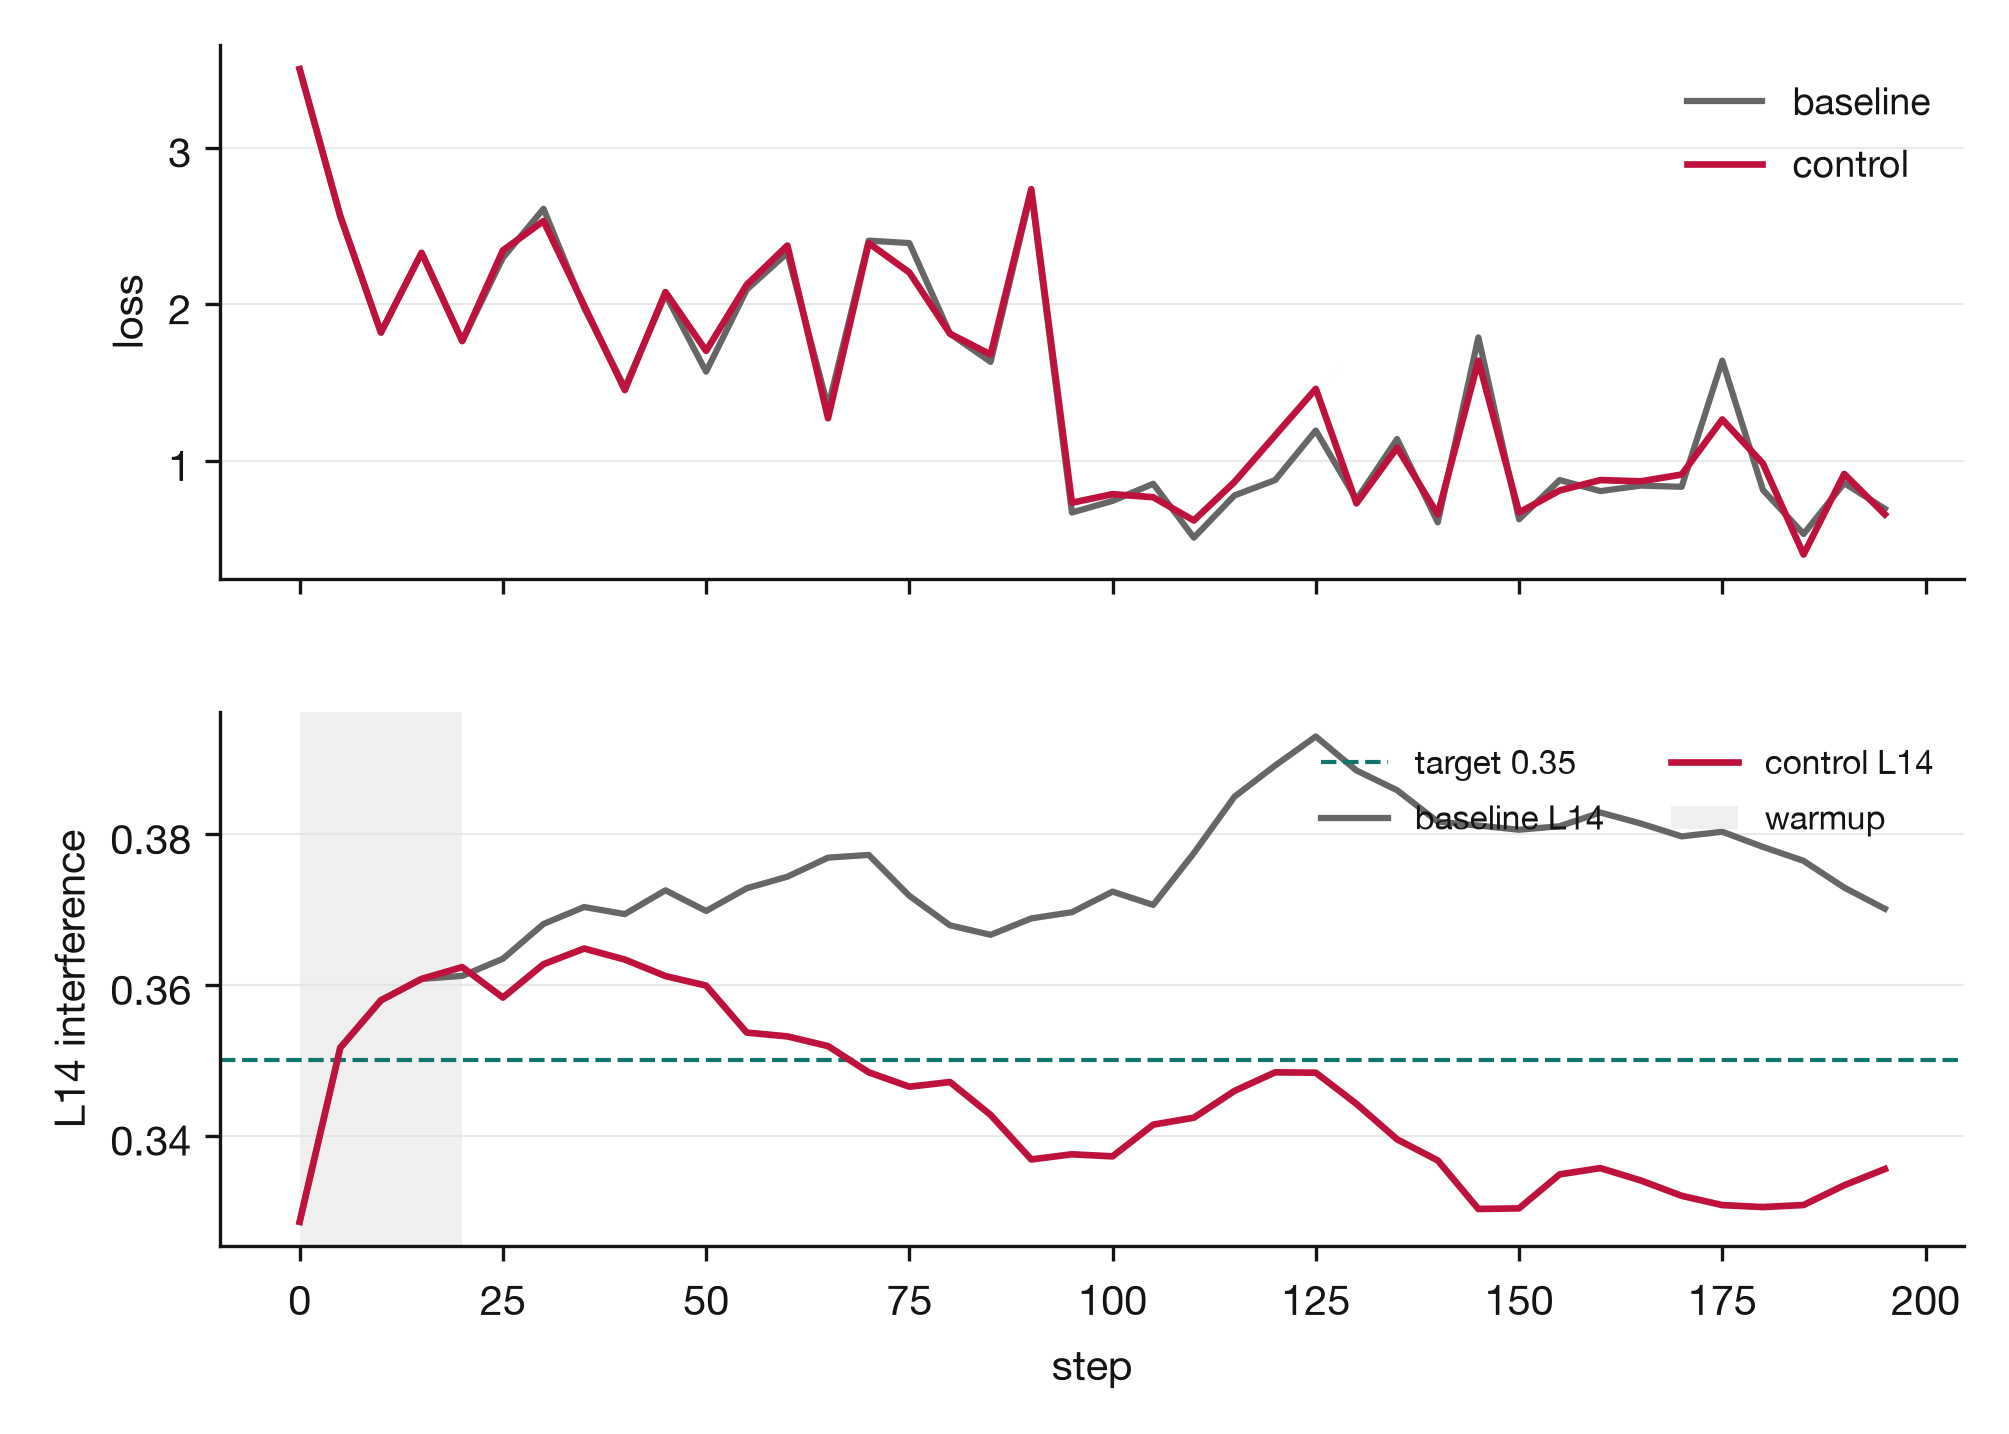
\includegraphics[width=\linewidth]{figures/fig02_control_vs_baseline.png}
  \caption{Matched control vs baseline (Qwen2.5-7B, seed $0$, $200$ steps). Soft
  regularizer on L14 interference toward $0.35$ after warmup; control ends
  closer to the packing target without collapsing loss.}
  \label{fig:control}
\end{figure}

Figure~\ref{fig:cards} summarizes the same pair as three cards.

\begin{figure}[H]
  \centering
  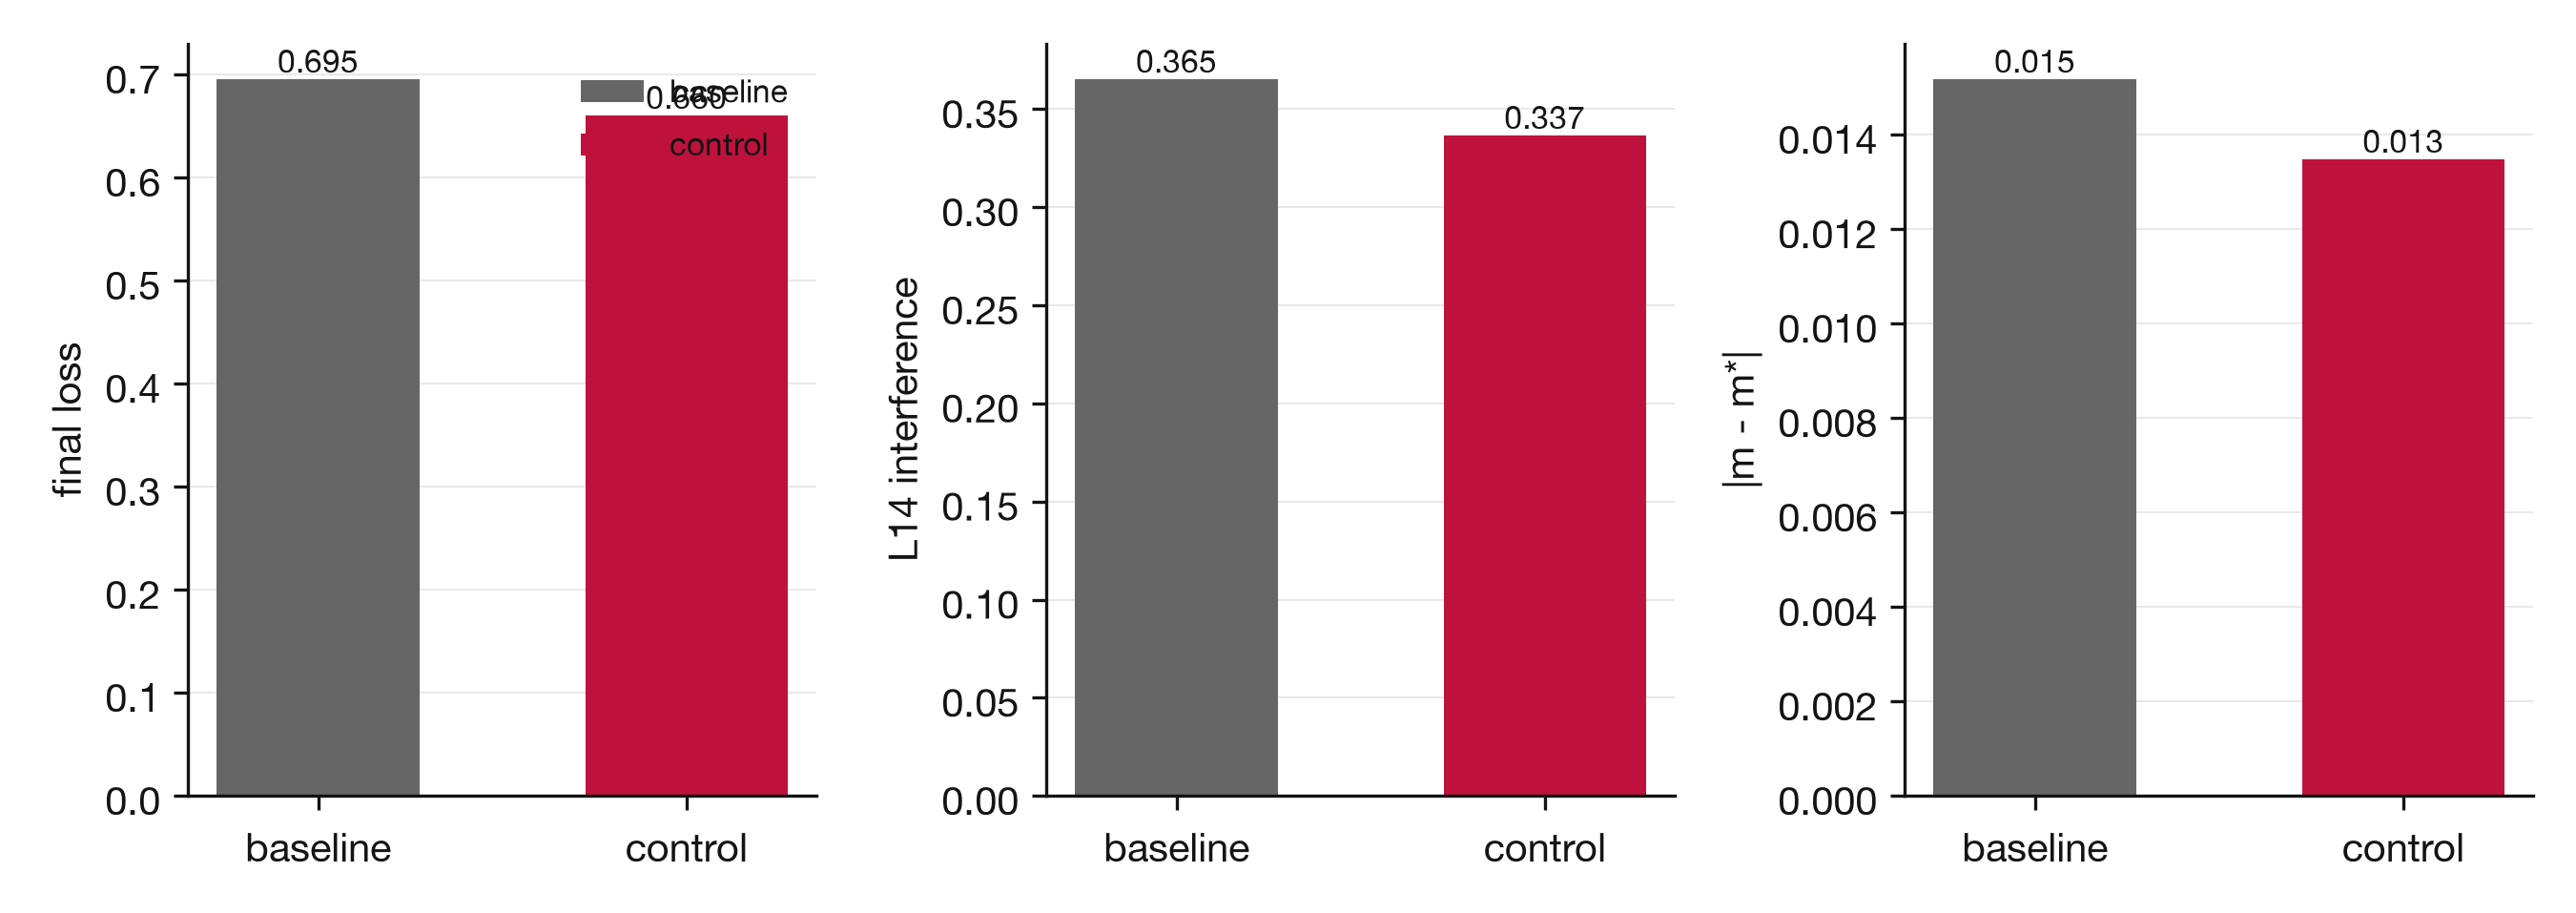
\includegraphics[width=0.95\linewidth]{figures/fig06_matched_pair.png}
  \caption{Summary cards for the matched pair: final loss, L14 interference,
  and absolute error to the packing target.}
  \label{fig:cards}
\end{figure}

\paragraph{Headline numbers.}
Baseline ends at L14 interference $0.365$ (error $0.015$ to target). Control
ends at $0.337$ (error $0.013$). Final LM loss on the logged curve is $0.695$
baseline vs $0.660$ control. Held-out eval loss improves under control
($2.075{\to}2.025$, $\Delta{=}{-}0.050$). The regularizer moved packing toward
$m^\star$ and improved generalization on this run.

\paragraph{Out-of-metric validation.}
We score the matched pair on checks that are not the training objective
(Table~\ref{tab:validation}): downstream loss stays healthy; related vs
unrelated structure holds under both runs; held-out probes stay clean; the
controlled trajectory still passes the same training-geometry checks as a
watch-only run. All seven claims pass.

\begin{table}[H]
  \centering
  \caption{Out-of-metric validation of soft control on the matched seed-$0$
  Qwen2.5-7B pair. All seven claims pass.}
  \label{tab:validation}
  \setlength{\tabcolsep}{4pt}
  \begin{tabular}{@{}llc@{}}
    \toprule
    Claim & Detail & Result \\
    \midrule
    Downstream loss &
      control $0.660$ vs baseline $0.695$ (slack $0.15$) &
      \textbf{PASS} \\
    Cross-feature (baseline) &
      related $0.037 < 0.5\times$ unrelated $0.280$ &
      \textbf{PASS} \\
    Cross-feature (control) &
      related $0.026 < 0.5\times$ unrelated $0.259$ &
      \textbf{PASS} \\
    Structure preserved &
      control still separates related vs unrelated &
      \textbf{PASS} \\
    Held-out not gamed &
      $|$train$-$heldout$|$ under cap &
      \textbf{PASS} \\
    Held-out not regressed &
      held-out L14 within slack of baseline &
      \textbf{PASS} \\
    Trajectory checks &
      training-geometry validate $6/6$ on control &
      \textbf{PASS} \\
    \bottomrule
  \end{tabular}
\end{table}

Soft control moves the live packing metric toward the target, keeps the watch
dashboard honest, and survives checks that are not the training objective.
That is a working knob.

\paragraph{Model scale.}
On the same extended corpus and seed, a smaller Qwen2.5-1.5B matched pair moves
toward $m^\star$ but loses on held-out LM loss ($\Delta{=}{+}0.063$). At 7B with
aligned banks and denser control, the pair hits packing \emph{and} held-out
($\Delta{=}{-}0.050$; Table~\ref{tab:scale}). Soft control is more useful where
there is capacity to spare.

\begin{table}[H]
  \centering
  \caption{Held-out LM loss: control minus baseline. Negative $\Delta$ means
  control wins. Extended corpus; matched LR and seed; $200$ steps.}
  \label{tab:scale}
  \setlength{\tabcolsep}{5pt}
  \begin{tabular}{@{}lcccc@{}}
    \toprule
    Model & Eval $\Delta$ & $|m{-}m^\star|$ base & $|m{-}m^\star|$ ctrl & Held-out \\
    \midrule
    Qwen2.5-1.5B & $+0.063$ & $0.072$ & $0.064$ & lose \\
    Qwen2.5-7B (m$\star$) & $-0.050$ & $0.015$ & $0.013$ & \textbf{win} \\
    \bottomrule
  \end{tabular}
\end{table}
\FloatBarrier

\section{How to read the signal}
\label{sec:limits}

A few rules make the dashboard sharper.

\paragraph{Bank relative.}
Every score is relative to the probe bank. Location probes make location
features look coherent. Freeze the bank in the checkpoint sidecar and reuse it
for diffs. Watch and control must share the same bank; a truncated control bank
reads as a false miss on $m^\star$.

\paragraph{Late layers and feature gaps.}
Late-layer spectra can swing harder than mid layers. Read relatedness at mid
layers; treat late-layer spectra as phase markers.

\paragraph{Corpus scale.}
The $200$-step extended corpus still admits memorization relative to public
pretraining corpora. Geometry still tracks the run
(Table~\ref{tab:scale}); larger public corpora are the next measurement step.

\paragraph{Train bank and held-out.}
The matched pair moves train-bank L14 toward target more than baseline. Held-out
probes stay within slack rather than chasing the same target, which is why
Table~\ref{tab:validation} checks outside the objective.

Use multi-layer watch, mid-layer diffs, frozen probes, and out-of-metric
checks as the standard read of a control run.

\section{Related work}

Toy superposition~\cite{elhage2022toy} and dictionary learning~\cite{bricken2023monosemanticity}
established that features share space. Spectral superposition theory~\cite{ivanov2026spectral}
and interference-weight models~\cite{olah2025interference} describe the
geometry of that sharing. Weight-editing work (ROME, MEMIT) rewrites facts in
MLP weights~\cite{meng2022rome,meng2023memit,geva2021ffn}; a thin edit demo
in our SDK shows the same geometry signal move when internals change. The gap
we fill is operational: treat geometry as a \emph{live training signal} you
track, diff, and softly steer beside loss.

\section{Conclusion}

Loss says how wrong. Geometry says how tangled. We put both on one dashboard,
show layer phases and feature structure on a Qwen2.5-7B fine-tune, and add a
soft regularizer that moves packing toward a target while improving held-out
loss, checked out-of-metric. Superposition geometry belongs beside loss. Soft
control is a knob you can turn.

Code, configs, and figure generators are public at
\url{https://github.com/Aquinf03/superposition-geometry-signal}
(\texttt{spg} SDK; regenerate figures with
\texttt{python experiments/paper\_figures.py}).

\section*{Acknowledgments}
This work was produced at Aquin Labs. Qwen2.5 checkpoints are released by
Alibaba Cloud under their model terms. Accept applicable licenses before
downloading weights.

\bibliographystyle{plain}
\bibliography{refs}

\end{document}
